\section{Results: Survey}
\label{section:Results_Survey}

\subsection{Population Selection}
We initially had two sources for our Experienced Drools users to send our survey to.
From LinkedIn we selected users who were at one degree of separation from us and listed Drools in their skills.
From StackOverflow we selected users who had asked or answered questions about Drools.

As in these two websites the users do not tend to list their contact details, some investigation was required.
From the initial selection, whose size we did not record we harvested email accounts, and failing that twitter accounts.

A few days into our survey we read a paper that described the use of academic papers as a population of expertise.
We used Google Scholar to look up Drools papers from the previous 2 years.
After skimming the papers to ensure that it was specifically about or using the Drools language we harvested emails

On the second and fourth day of the survey two subjects forwarded the weblink to the survey to mailing lists.
One, a developer from the core Drools team, sent it to a list of known Drools consultants.
The other sent it internally in his company.
both the subjects who sent the survey to their mailing list forwarded links to version C of the survey.

We had created 4 versions of the questionnaires to a combat single source bias.
We distributed the surveys to the subjects harvested from LinkedIn and StackOverflow evenly.
Because of the overrepresentation of Survey C, we distributed the subjects harvested from academic papers evenly over Surveys A, B and D.

The collection result can be seen in figure \ref{fig:Survey_participants}.
What we see here is that the method of collection did not have much of an impact on return rates.
whilst StackOverflow had a higher rate, the number of people contacted was so small that a small addition of respondents has an outsized effect on the proportion.

The first three pie charts represents the collection methods over which we had control.
These three represented 24 of our 30 completed questionnaires.
The last pie chart represents 6 completed and 4 partially completed questionnaires, that were returned from the surveys sent on by our initial participants.
We do not know the size of the starting population of these lists. 
Thus this pie chart only shows the ratio of partial to completed results.


In summary, a survey reached known 154 participants, of which 24 completed it, for a Response Rate of 15.5\%.
In addition, an unknown amount of participants were reached through mailing lists, returning a further 6 completed surveys.

\subsection{Participant Demography}

Responses came from around the world.
Figure \ref{fig:Survey_locations} shows the location of the respondents were concentrated in Europe, the exceptions being the USA, Israel, and Singapore.
Italy and the Netherlands provided the largest number of responses, with 7 and 5 respectively.

\begin{figure}[H]
    \centering
    \fbox{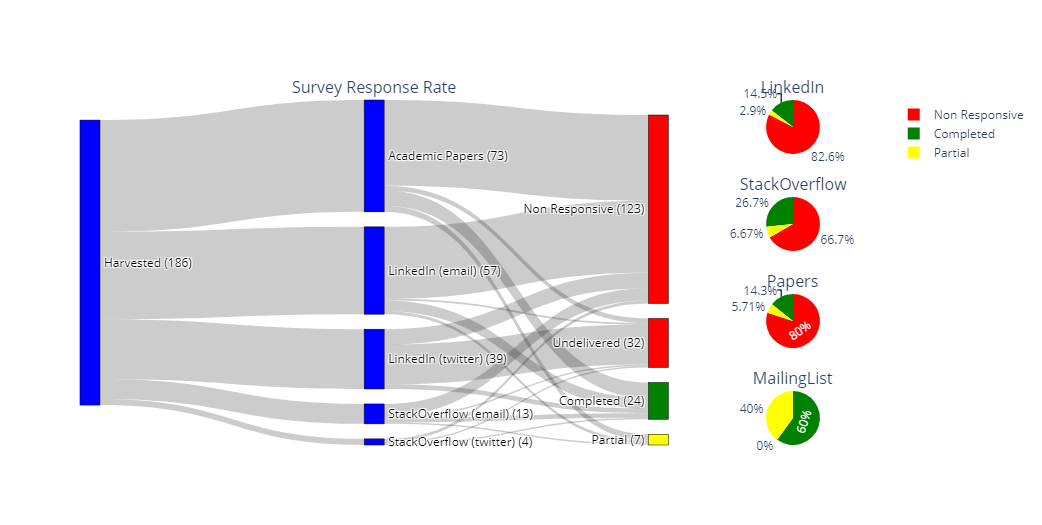
\includegraphics[width=0.95\textwidth]{Sections/images/survey_participants.png}}
    \caption{Survey participants}
    \label{fig:Survey_participants}
\end{figure}

\begin{figure}[H]
    \centering
    \fbox{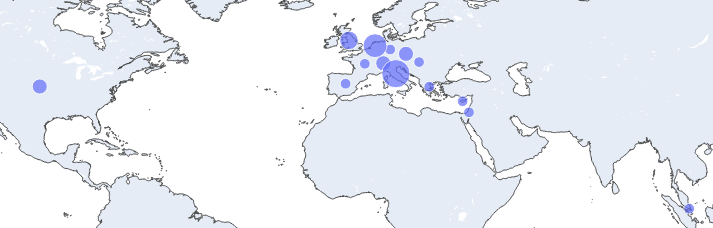
\includegraphics[width=0.95\textwidth]{Sections/images/survey_locations.png}}
    \caption{Survey locations}
    \label{fig:Survey_locations}
\end{figure}

\begin{figure}[H]
    \begin{subfigure}{.33\textwidth}
      \centering
      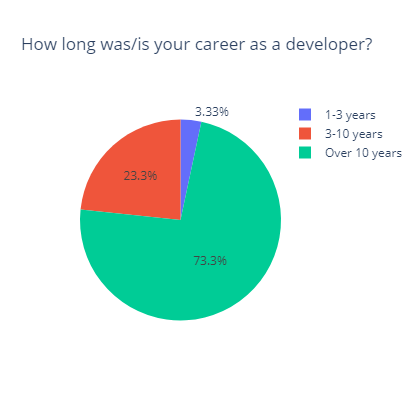
\includegraphics[width=.95\linewidth]{Sections/images/pie_experiencer.png}
      \caption{SE experience}
      \label{fig:sfig1}
    \end{subfigure}%
    \begin{subfigure}{.33\textwidth}
      \centering
      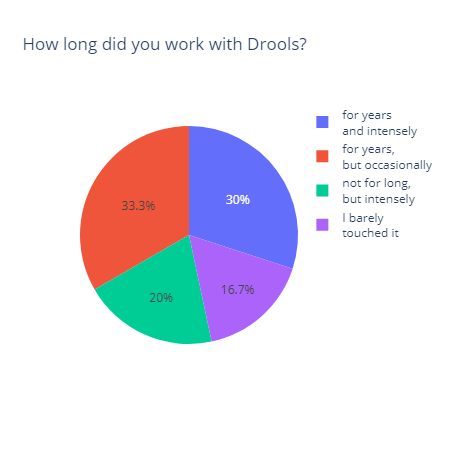
\includegraphics[width=.95\linewidth]{Sections/images/pie_droolsExperience.png}
      \caption{Drools experience}
      \label{fig:sfig2}
    \end{subfigure}
    \begin{subfigure}{.33\textwidth}
        \centering
        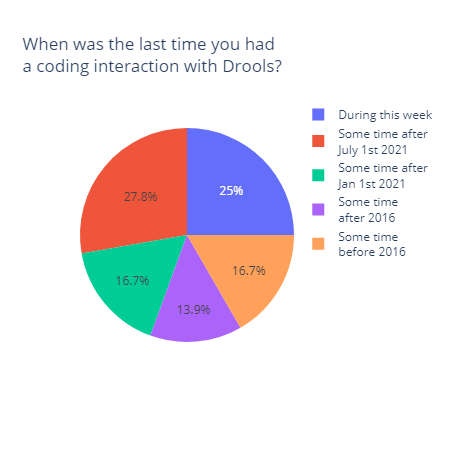
\includegraphics[width=.95\linewidth]{Sections/images/pie_recentusage.png}
        \caption{Recent use}
        \label{fig:sfig3}
      \end{subfigure}
    \caption{Subject experience}
    \label{fig:subject_experience}
\end{figure}

The experience of our subjects was quite high.
As can be seen in \ref{fig:sfig1}, most of our subjects have over 10 years programming experience.
17\% of our recipients had a low experience of Drools, and 30\% were very experienced, as shown in figure \ref{fig:sfig2}.
Figure \ref{fig:sfig3} reports that over half of our recipients have used Drools in the previous 6 weeks with only 17\% not having used Drools for more than 5 years.

Half of our subjects reported only ever using one editor for Drools, with the slight majority of those only using Eclipse.
Eclipse also had the most instances of reporting of having been used, out of the 55 instances of editors reported as being used, 20 of those were Eclipse.
There was a, to us, surprising diversity of tools being used.
The purpose of this section was to be able to calibrate responses against exposure to IDEs with greater Drools Support.
The wide diversity of editor usage and high incidence of multiple editor usage means that these answers are not suitable for use in the sub-categorisation of responses. 
The distribution of usage is shown in figure \ref{fig:editorUsage}.

\begin{figure}[h]
    \centering
    \fbox{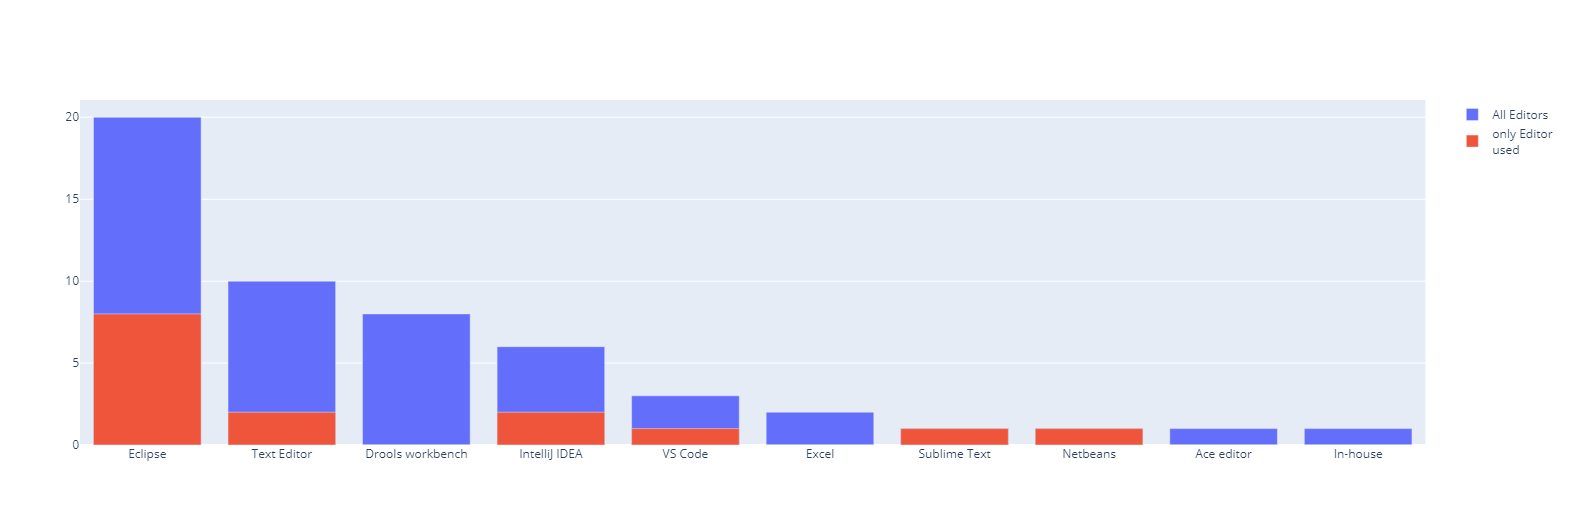
\includegraphics[width=0.95\textwidth]{Sections/images/EditorUseage.png}}
    \caption{Editors used}
    \label{fig:editorUsage}
\end{figure}


\subsection{Question Analysis}
Until now, the choice of chart to display the survey outcome has been based on a feeling rather than research. 
The remainder of this Results sections, whilst talking about results that regard our Likert Scaled questions, we will be following the advice of Robbins et.al.\cite{robbins2011plotting} and using diverging stacked bar charts, with counts added.
This style allows the evaluation of subclasses results.
The addition of counts makes it easier to spot when the results are skewed by small numbers.

When displaying subtypes we shall split into groups.
The source of the response will create a pseudo cross-section of our participants.
The 10 who were contacted through academic papers will be considered our academics.
The remaining 20 will be considered practitioners.

The next grouping will be on Drools Experience.
The 9 who replied they had used drools ``for years and intensely'' are categorised as experts.
The 16 who either answered ``for years, but occasionally'' or ``not for long, but intensely'' are categorised as seniors.
The 5 who answered ``I barely touched it'' are categorised as novices.

Another grouping will be on recency of use.
The 12 who have used Drools in 2021 will be categorised as current users.
The remaining 18 as past users.

To remove some bias in the questionnaires we changed question order, order of projections, and which rulesets were used.
When a question is effected by this, then this will also be displayed.

\subsubsection{Question 1, 2 and 3: First Impressions}

\begin{figure}[H]
    \centering
    \fbox{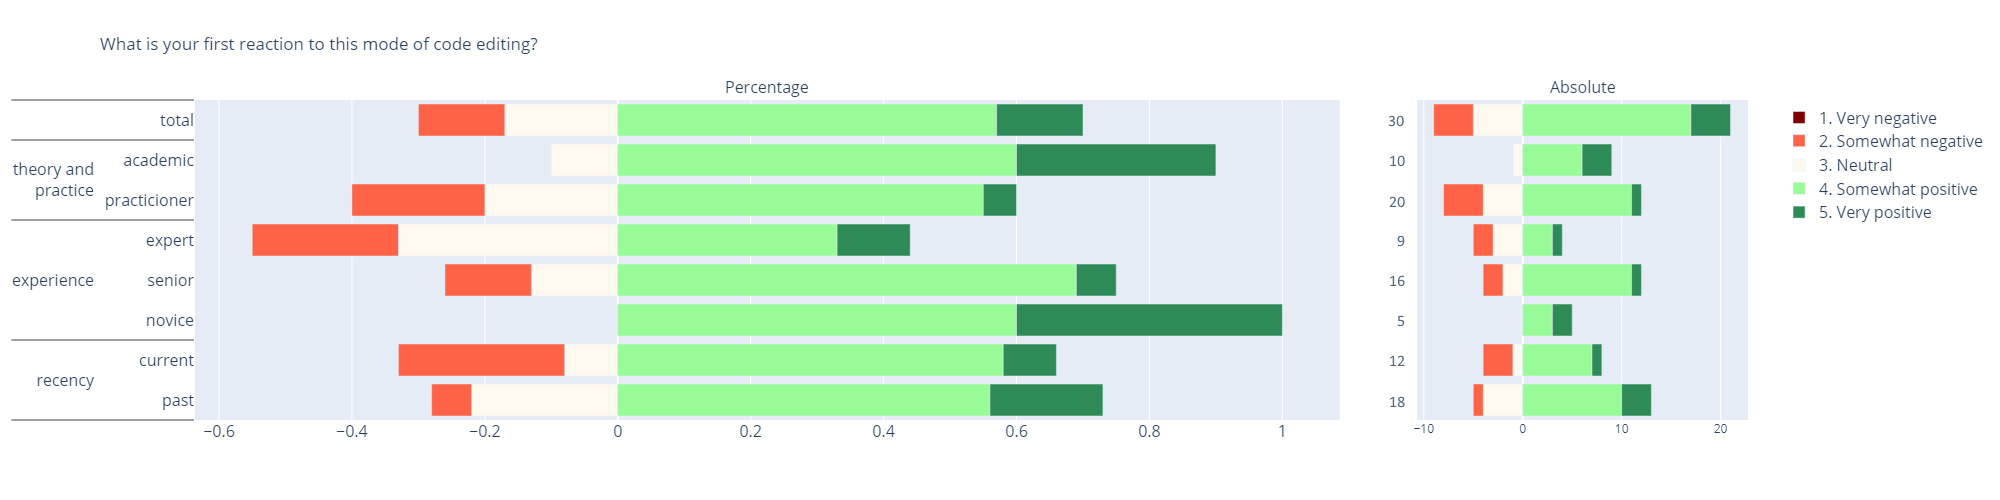
\includegraphics[width=0.95\textwidth]{Sections/images/stackedbar_Q1.png}}
    \caption{Question 1 - first impressions}
    \label{fig:stackedbar_Q1}
\end{figure}

This question shows the subject an example of projectional editing a Drools file alongside a table projection, as an animated GIF, along with an explanation.
Then she is asked her first reaction. The chart in figure \ref{fig:stackedbar_Q1} shows the outcomes.

We see far more positive than negative answers here.
Those who had a positive or negative responses were directed to answer the open questions ``Q2. How would this coding style be useful to your interactions with Drools?'' and ``Q3. What do you find negative with this style of coding?'' respectively.
Figure \ref{fig:wordclouds} show a not very useful, but funky looking visualization of the subjects responses.

\begin{figure}[H]
    \begin{subfigure}{.60\textwidth}
      \centering
      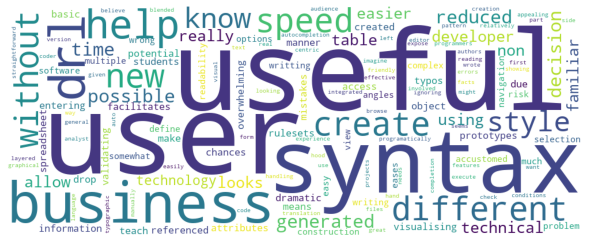
\includegraphics[width=.95\linewidth]{Sections/images/positive_wordcloud.png}
      \caption{Positive}
      \label{fig:wfig1}
    \end{subfigure}%
    \begin{subfigure}{.40\textwidth}
      \centering
      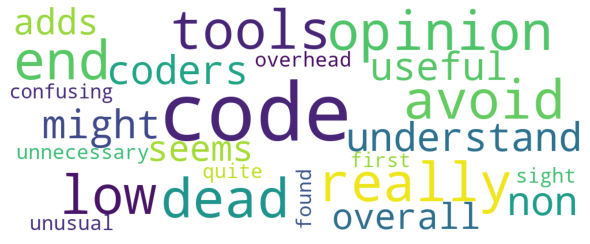
\includegraphics[width=.95\linewidth]{Sections/images/negative_wordcloud.png}
      \caption{Negative}
      \label{fig:wfig2}
    \end{subfigure}
    \caption{Initial thoughts}
    \label{fig:wordclouds}
\end{figure}

An observation that can be taken is that the novice and the academics (where there is a lot of crossover), found the initial presentation more positive than the experienced practitioners.
It should be noted that these are groups with a size of 10 and 5, so their statistical use is not very high.
A trend however can be seen from experts finding

As can be seen in this question an consistent with the other questions, whether a person is a current or a past user of drools makes not have a significant impact on their responses.

Amongst the positive comments it appears the the subjects had all picked up on many of the advantages that projectional editing brings.
The ones that got the most mentions, using other words, were exploratory coding, correctness by construction, and multiple viewpoints.
It was also noted, with the projections shown, that development could be quicker and easier to check.

Amongst the, very few, negative comments, they discussed the failures of no/low code solutions, that the view was confusing and they felt it added unnecessary overhead.

\pagebreak
\subsubsection{Question 4 and 5: Interpret Projection}

\begin{figure}[H]
    \centering
    \fbox{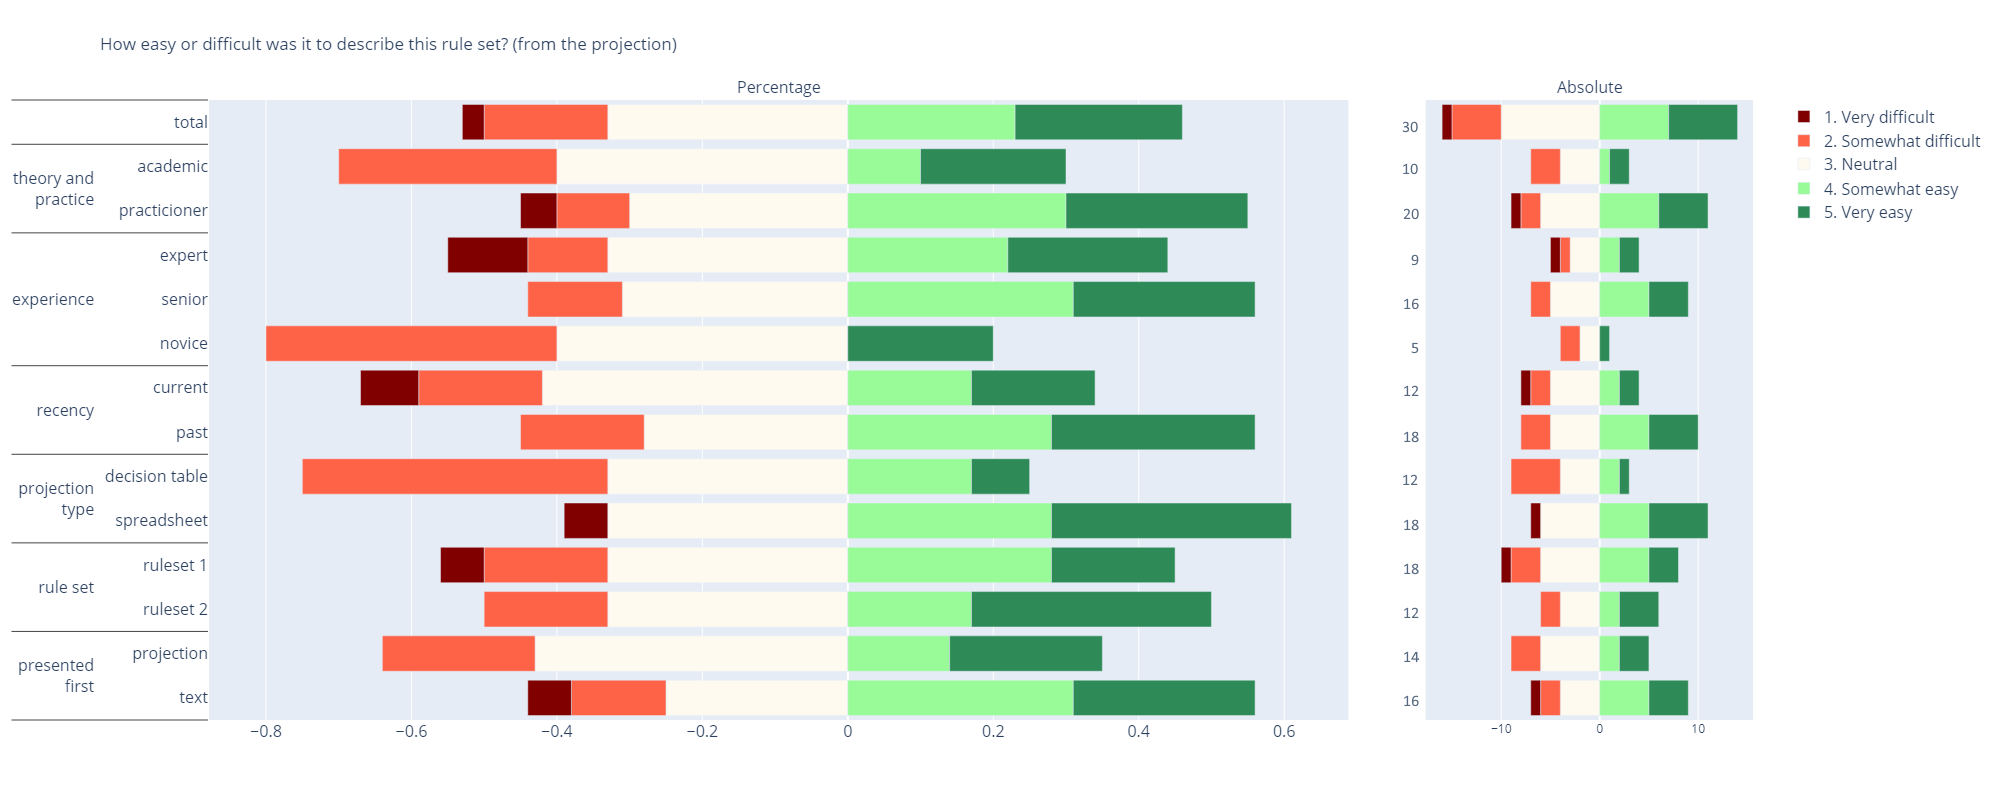
\includegraphics[width=0.95\textwidth]{Sections/images/stackedbar_Q2.png}}
    \caption{Question 5 - interpret projection}
    \label{fig:stackedbar_Q2}
\end{figure}

This question asks the subject to describe the meaning of the projection and then describe how hard it was to do that.
Very few people described it well.
There was a distinct difference between the participants belief that they understood the ruleset between the projections presented.
The participants believed they understood the spread sheet style projection better then the decision table projection.

There was not a notable difference between rulesets presented and whether they were presented text first or the projection first.

There was one extreme response, which was negative.
This came from an expert practitioner who saw the text version before seeing the projection.


\subsubsection{Question 6 and 7: Interpret Text}

\begin{figure}[H]
    \centering
    \fbox{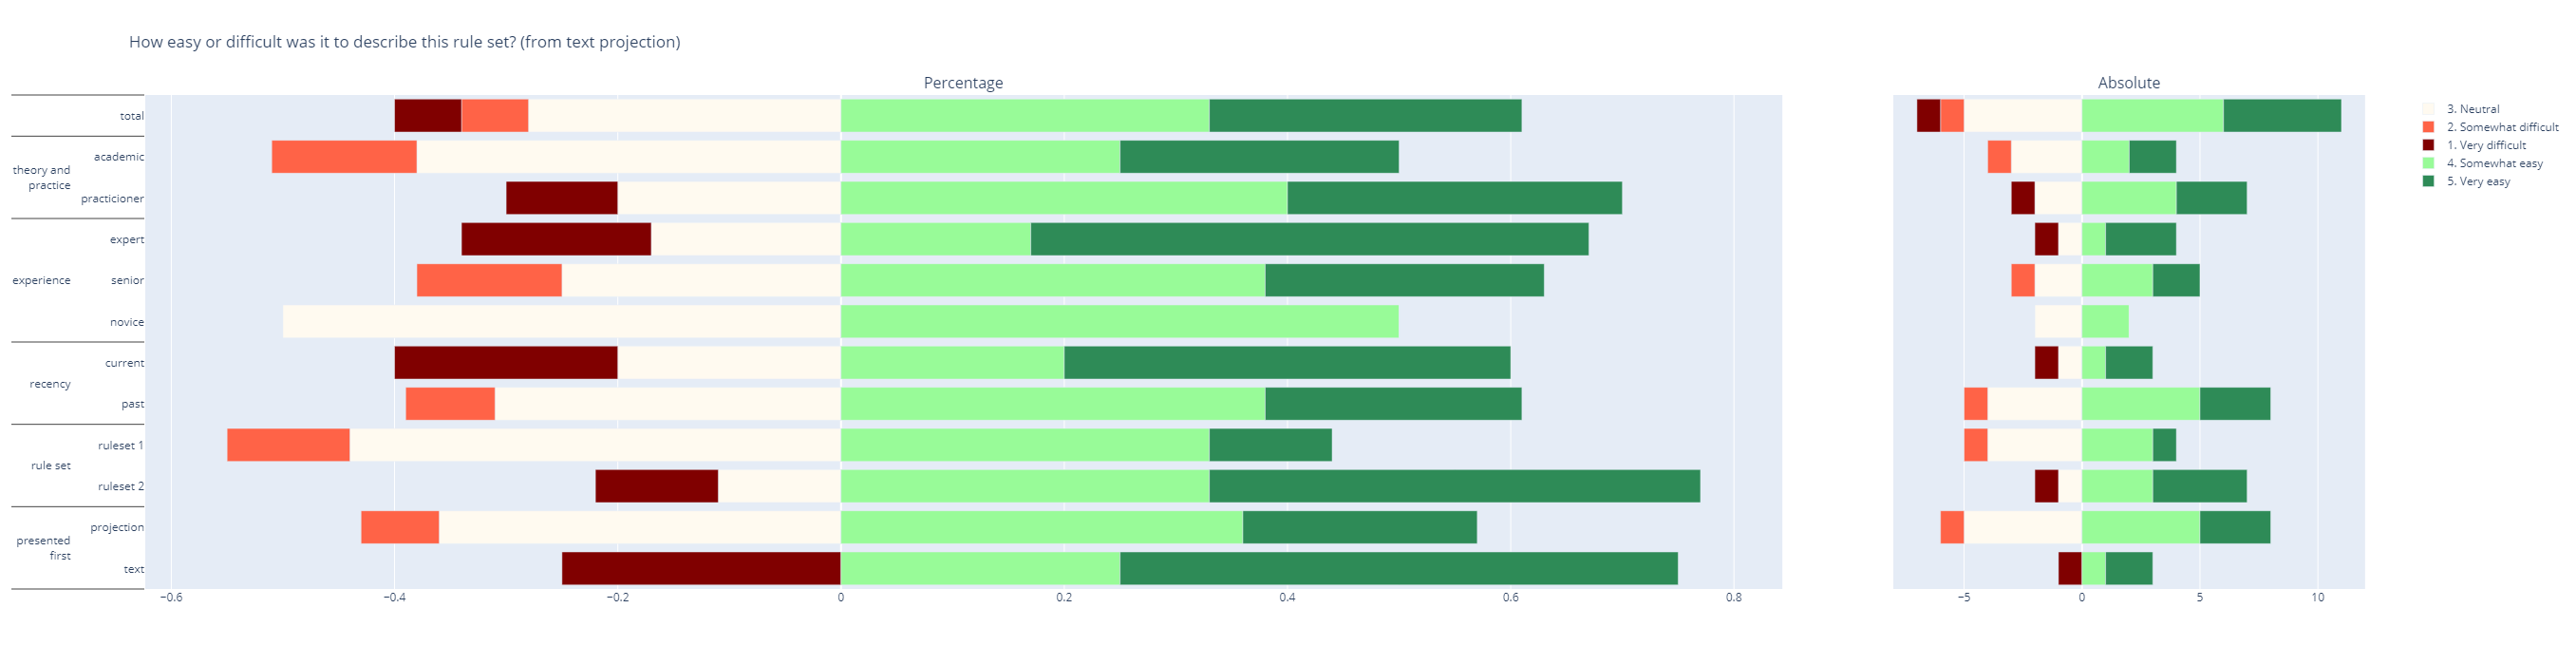
\includegraphics[width=0.95\textwidth]{Sections/images/stackedbar_Q3.png}}
    \caption{Question 7 - interpret text}
    \label{fig:stackedbar_Q3}
\end{figure}

This question asks the subject to interpret a rule set that is presented in a Drools style text projection.
The purpose of this question was three fold.
First, to calibrate how well the subject really understood drools.
Second, for a comparison with with a later projection.
Finally, to calibrate whether and how much easier the text was than the projection to those used to seeing the text version.

Unfortunately, we assume due to the questionnaire design, there was a large number of non-respondents to this question. 
12 of the 30 respondents did not answer this question.
All 12 of these were from the 16 that were presented the text projection before the tabular projections.

Reporting on 18 responses has a lot less validity.
With that in mind we do see that there a greater belief in the participants that they understood the meaning of the text projections better than they did the tabular projections.

\subsubsection{Question 8: Compare Projections}

\begin{figure}[H]
    \centering
    \fbox{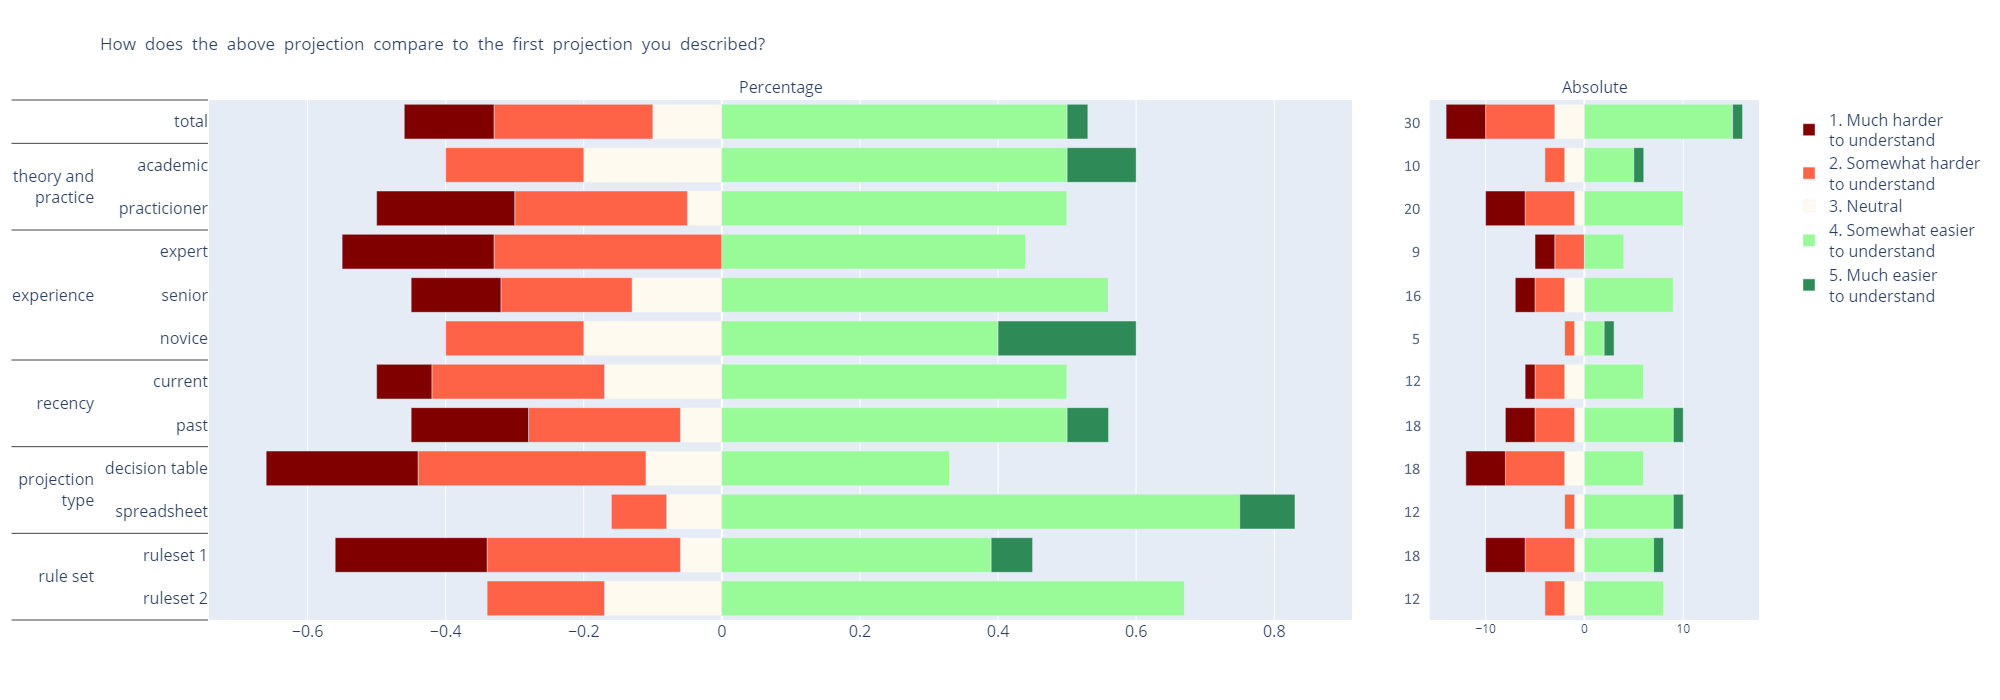
\includegraphics[width=0.95\textwidth]{Sections/images/stackedbar_Q4.png}}
    \caption{Question 8 - compare projections}
    \label{fig:stackedbar_Q4}
\end{figure}

This question asked the participant to compare the two tabular projections.  
This question was to calibrate whether one projection was considerably worse than the other and whether that would affect the comparison with text.

In these results the total does not matter, it is only which projection type and which rule type which can have a meaningful effect.
The results show that the spreadsheet style projection is considered much more understandable than the decision table style projection.
There was also a slightly negative effect of rule set 1 over rule set 2, which surprised us, because we considered rule set 1 to be simpler.

\subsubsection{Question 9: Compare Projection to Text}

\begin{figure}[H]
    \centering
    \fbox{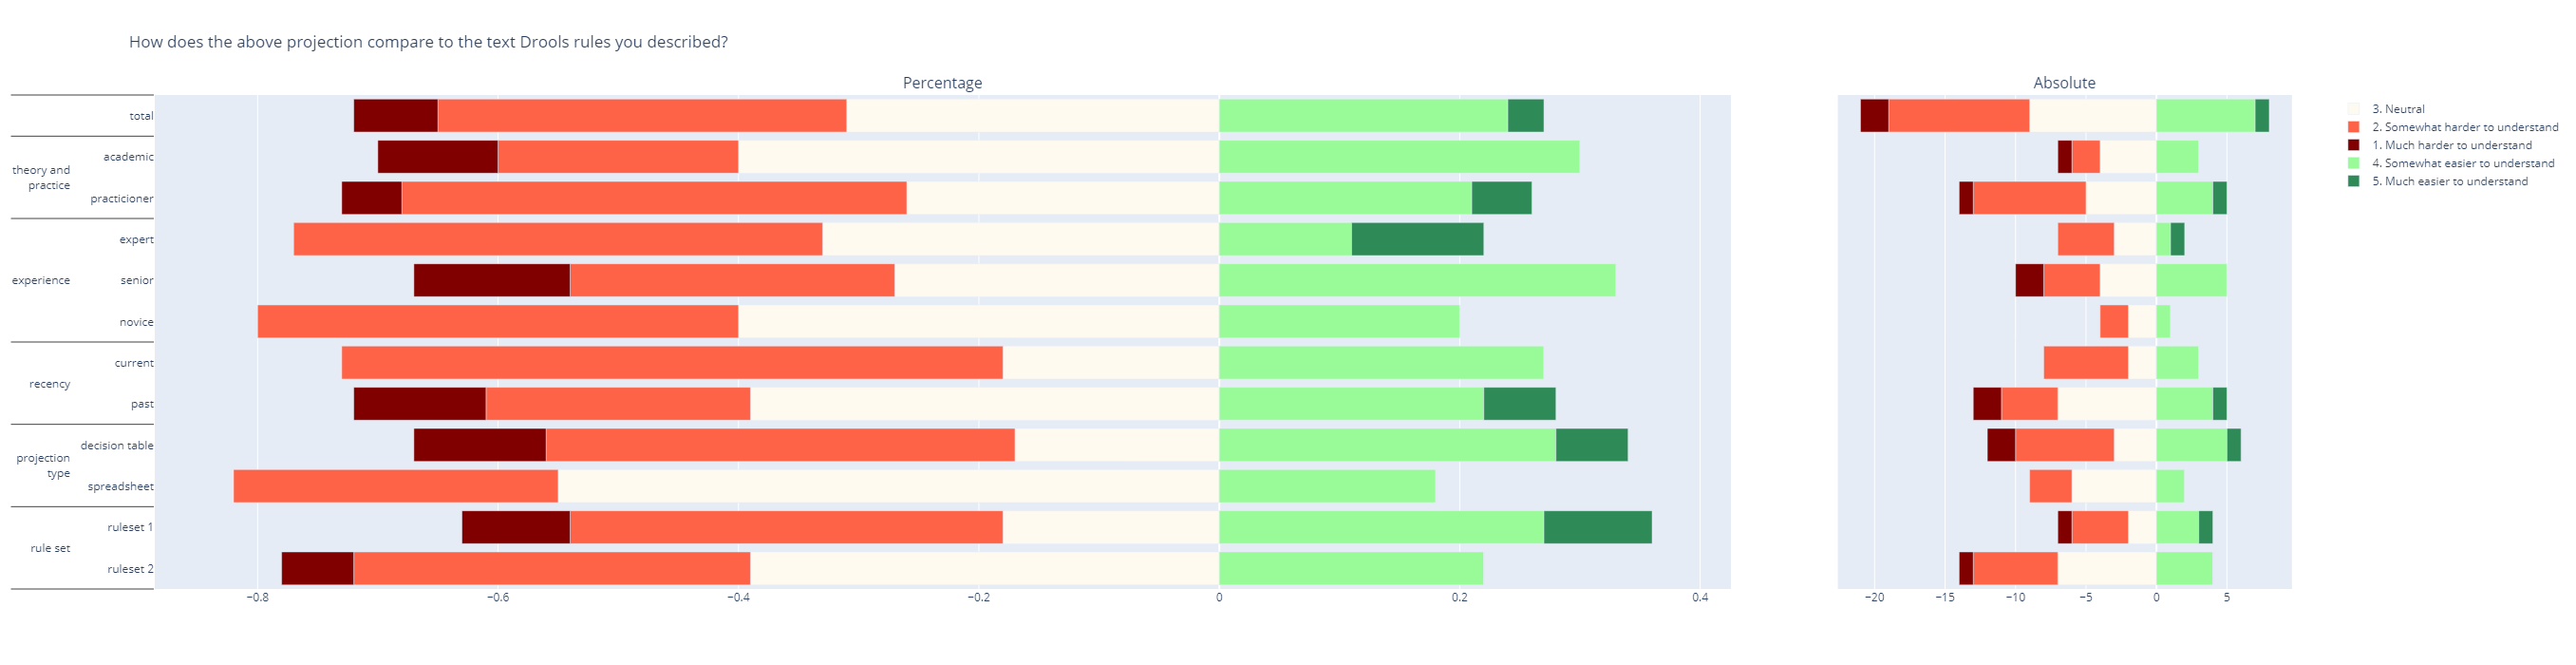
\includegraphics[width=0.95\textwidth]{Sections/images/stackedbar_Q5.png}}
    \caption{Question 9 - compare projections with text}
    \label{fig:stackedbar_Q5}
\end{figure}

This question asked our subjects to compare a tabular projection with the text projection.
There was one participant that chose not to answer this question.

This result was pretty definitive.
The subjects, independent of any other factors, found very much that the textual projections were more understandable than the tabular projections.

\subsubsection{Question 10: Truth Table Validation}

\begin{figure}[H]
    \centering
    \fbox{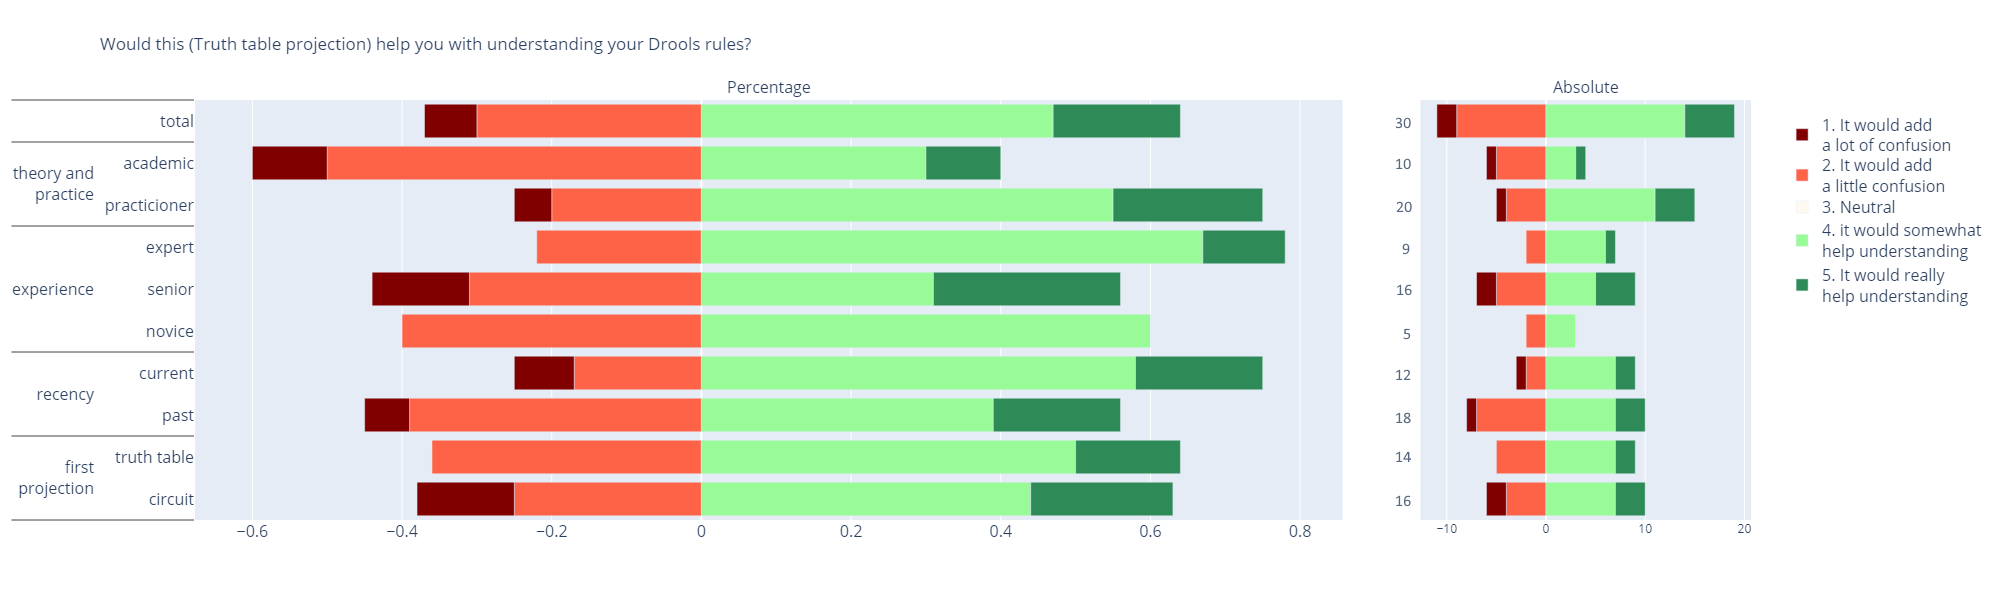
\includegraphics[width=0.95\textwidth]{Sections/images/stackedbar_Q6.png}}
    \caption{Question 10 - truth table}
    \label{fig:stackedbar_Q6}
\end{figure}

This question presented the subject with a wireframe of a truth table.

The results given were dichotomous.
Every subject had a positive or negative view of the projection.
0 of the 30 subjects gave a neutral result.
This was an unlikely result.

There was a very positive view of this projection.
Experts found this view particularly good.
Academics offered the most negative view of this projection.

Whilst the positive side was highly positive than the, the negatives views were also higher than normal. 

\subsubsection{Question 11: Circuit Diagram Validation}

\begin{figure}[H]
    \centering
    \fbox{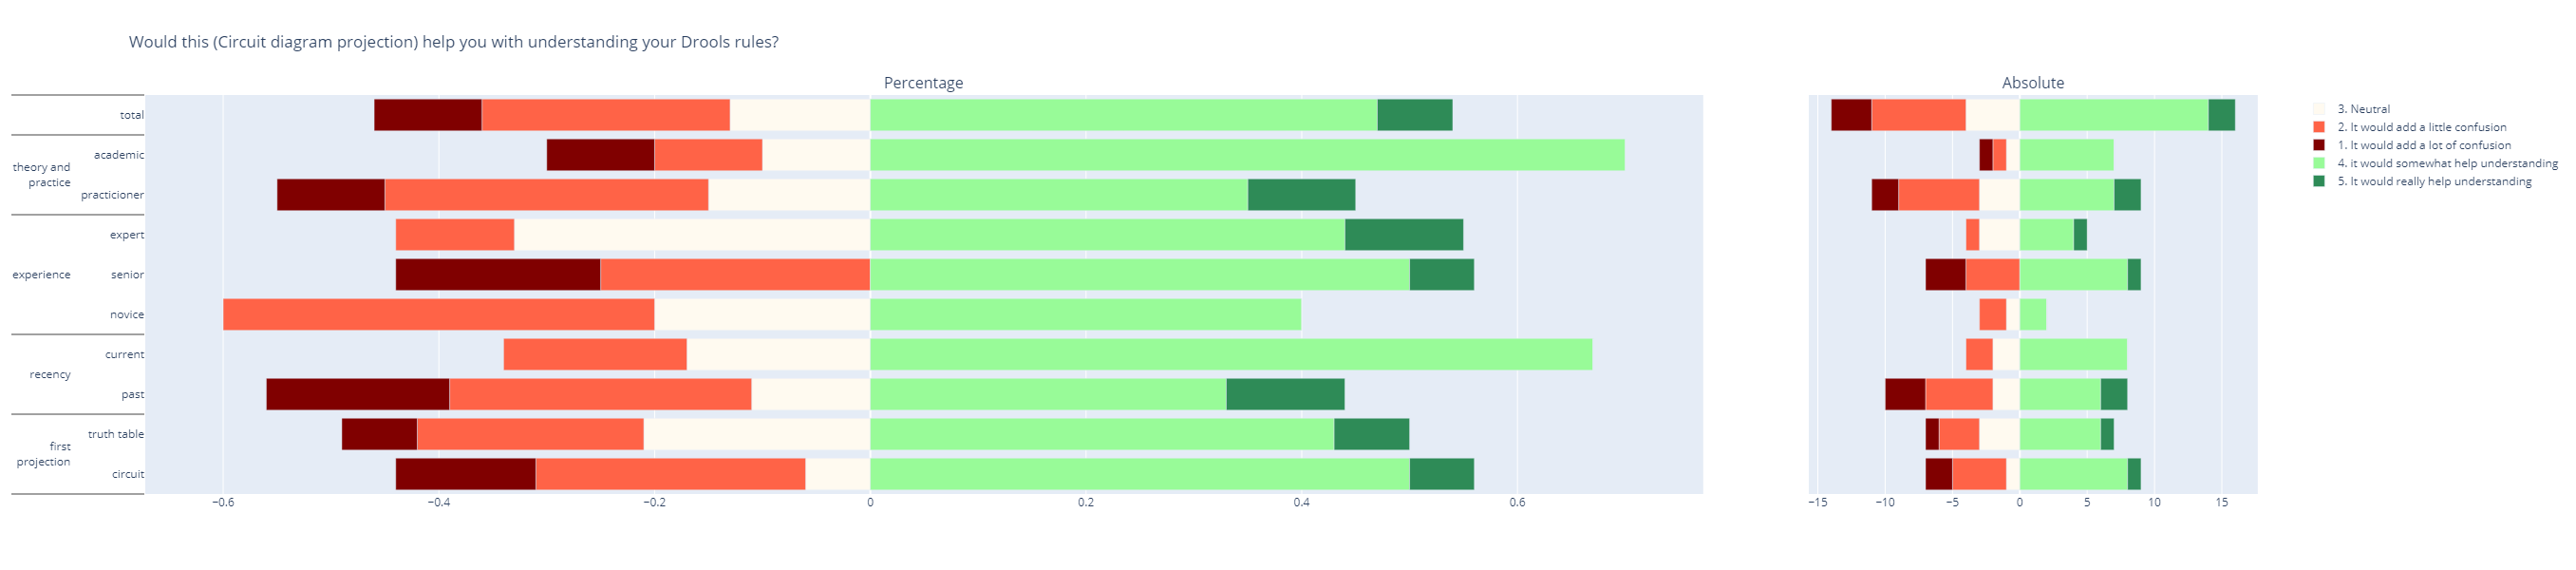
\includegraphics[width=0.95\textwidth]{Sections/images/stackedbar_Q7.png}}
    \caption{Question 11 - circuit diagram}
    \label{fig:stackedbar_Q7}
\end{figure}

This question presented the subject with a wireframe of a circuit diagram.

The view of the circuit diagram was pretty evenly distributed between positive and neutral or negative views.

\subsubsection{Question 15: Closing Remarks}

Our last question asks for any last comments.
16 participants decided to add some words.

We ran sentiment analysis on these 16 comments.
9 were considered positive, 6 mixed and 1 negative.
Figure \ref{fig:Q15_wordcloud} shows a funky little word cloud, because why not! [TODO: rewrite when sober]

\begin{figure}[H]
    \centering
    \fbox{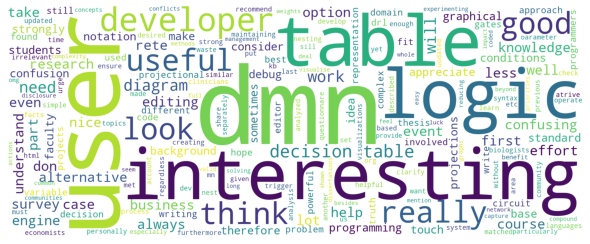
\includegraphics[width=0.95\textwidth]{Sections/images/Q15_wordcloud.png}}
    \caption{Question 15 - responses}
    \label{fig:Q15_wordcloud}
\end{figure}

